\documentclass[11pt]{article}
\usepackage[margin=1.5in]{geometry}
\usepackage{graphicx}
\usepackage{float}
\usepackage{parskip}
\usepackage{amsmath}

\usepackage{pgfplots}
\pgfplotsset{width=10cm, compat=1.9}
\usepgfplotslibrary{external}
\tikzexternalize

\begin{document}

\textbf{\Huge Functions}

Athan Zhang \& Jeffrey Chen

\section{Understanding Functions}

A function is a mathematical rule that assigns a unique output to each input. It represents a relationship where each input value corresponds to exactly one output value. We often use the notation $f(x)$ to denote a function, where $f(x)$ represents the function name and $x$ represents the input variable. This is read as "f of x" and interpreted as the value of the function f at x.

\subsection{Domain and Range}

The \textbf{domain} of a function represents the set of all possible input values for which the function is defined. For example, consider a function $f(x)$ that calculates the square root of $x$. In this case, the domain of $f(x)$ would be all real numbers greater than or equal to zero since the square root of a negative number is not defined within the real number system.

On the other hand, the \textbf{range} of a function represents the set of all possible output values that the function can produce. It describes the set of values that the function "hits" or reaches. For the same example function $f(x)$, the range would be all real numbers greater than or equal to zero, as the square root of a non-negative number always yields a non-negative result.

\subsection{Interval Notation}

Interval notation uses inequalities to describe subsets of real numbers. The symbols [ or ] (square brackets) and ( or ) (parenthesis) are commonly used to indicate endpoints of an interval. Square brackets are inclusive and mean that the number at that endpoint is included in the interval. In contrast, parenthesis are exclusive, meaning that the number at the endpoint is NOT included in the interval.

\begin{table}[H]
\centering
\begin{tabular}{|cc|cc|}
\hline
\multicolumn{2}{|c|}{Bounded Interval} & \multicolumn{2}{c|}{Unbounded Interval} \\ \hline
\multicolumn{1}{|l|}{Inequality} & \multicolumn{1}{l|}{Notation} & \multicolumn{1}{l|}{Inequality} & \multicolumn{1}{l|}{Notation} \\ \hline
\multicolumn{1}{|c|}{$a \leq x \leq b$} & {[}a, b{]} & \multicolumn{1}{c|}{$x \geq a$} & $[a, \infty)$ \\
\multicolumn{1}{|c|}{$a < x < b$} & (a, b)     & \multicolumn{1}{c|}{$x \leq a$} & $(-\infty,a{]}$  \\
\multicolumn{1}{|c|}{$a \leq x < b$} & {[}a, b)   & \multicolumn{1}{c|}{$x > a$} & $(a, \infty)$   \\
\multicolumn{1}{|c|}{$a < x \leq b$}& (a, b{]}& \multicolumn{1}{c|}{$x < a$} & $(-\infty, a)$\\
\multicolumn{1}{|c|}{}           &                               & \multicolumn{1}{c|}{$-\infty < x < \infty$}          & $(-\infty, \infty)$                            \\ \hline
\end{tabular}
\end{table}

Finally, union notation is a commonly used method to describe unions of subsets and sets. It is denoted as the symbol $\cup$. For example, $[1, 3)\cup(3, 5]$ represents all real numbers from $1$ to $5$ inclusive, except for $3$. Interval notation and union notation are often used together to describe the domain and range of certain functions.

\subsection{Function Representation}

Functions can be represented in various ways. This includes:

\begin{itemize}
    \item \textbf{Algebraically:} An equation relating x- and y-coordinates or each point. Note: there is some degree of nuance present here, as not every curve that can be represented with an equation is a function, such as a circle.
    \item \textbf{Graphically:} Points on a graph in the coordinate plane represent the points.
    \item \textbf{Numerically:} A table of values or a set of points relates each input (x-value) with an output value (y-value)
    \item \textbf{Verbally:} A sentence describes how the inputs and outputs are related.
\end{itemize}



\section{Continuity and Limits}

% expand more later
% an image would be nice here
\subsection{Limits}
A \textbf{limit} refers to the value that a function's output approaches as the input approaches a specific number. It describes the behavior of a function at a point of interest. The limit of $f(x)$ as $x$ approaches $x_0$ is written using the following notation: $\lim_{x\to x_0} f(x)$. 

Limits can be taken from both the \textbf{left} and \textbf{right} hand sides. This means analyzing the behavior of $f(x)$ as $x$ approaches a certain value from the left hand side alone, or from the right hand side alone. This is important as sometimes these values differ, creating results that will be explained further in the following sections. 

The left hand limit of $f(x)$ as $x$ approaches $x_0$ is written as $\lim_{x\to x_0^-} f(x)$. Similarly, the right hand limit of $f(x)$ as $x$ approaches $x_0$ is written as $\lim_{x\to x_0^+} f(x)$. It is said that $\lim_{x\to x_0} f(x)$ \textbf{exists} when $\lim_{x\to x_0^-} f(x) = \lim_{x\to x_0^+} f(x)$ and \textbf{does not exist} when $\lim_{x\to x_0^-} f(x) \neq \lim_{x\to x_0^+} f(x)$.

\subsection{Continuity}
A function is called \textbf{continuous} when it has no abrupt interruptions in its behavior. Simply put, a continuous function can be drawn with a single, unbroken curve. 

More rigorously speaking, there are 3 requirements for a function $f(x)$ to be continuous at any given point $x_0$: 
\begin{itemize}
  \item $\lim_{x\to x_0} f(x)$ must exist.
  \item $f(x)$ must be defined at $x_0$.
  \item $\lim_{x\to x_0} f(x)$ must equal $f(x_0)$.
\end{itemize}

Sometimes, a function may be continuous except for one or more specific points. These points are referred to as \textbf{discontinuities}.

\subsection{Types of Discontinuities}
There are generally 4 types of discontinuities: jump discontinuities, infinite discontinuities, hole discontinuities, and endpoint discontinuities. 

\subsubsection*{Jump Discontinuities}
A jump discontinuity is defined as a point on a function where the limits from the right and left hand side are not equal. This occurs most of the time with piecewise functions.

\begin{center}
\begin{tikzpicture}
\begin{axis}[
    axis lines=middle, width=6cm, height=6cm
]
\pgfplotsset{hole/.style={color=red,fill=white,only marks,mark=*}}
\pgfplotsset{dot/.style={color=red,fill=red,only marks,mark=*}}
\addplot[domain=-4:1, color=red]{x};
\addplot[domain=1:4, color=red]{x+1};
\addplot[hole] coordinates{(1,1)};
\addplot[dot] coordinates{(1,2)};
\end{axis}
\end{tikzpicture}
\end{center}

\subsubsection*{Infinite Discontinuities}
An infinite discontinuity is defined as a point on a function where the limits from the right and left hand side approach $\pm\infty$. This occurs most of the time when dividing by $0$.

\begin{center}
\begin{tikzpicture}
\begin{axis}%
    [ 
        xmin=-4,
        xmax=4,
        axis x line=middle,
        ytick={-4, -2, 2, 4},
        ymin=-4,
        ymax=4,
        axis y line=middle,
        samples=100,
        domain=-10:10,
        restrict y to domain=-30:30,
        width=6cm, height=6cm
    ]
    \addplot[thick,samples=400, color=red] (x,{1/x});
\end{axis} 
\end{tikzpicture}
\end{center}

\subsubsection*{Hole Discontinuities}
A hole discontinuity is defined as a point on a function where the limit exists, but the function itself is not defined, or does not equal the limit. These discontinuities are referred to as "removable" due to the fact that they can often be removed from the function with a bit of algebraic manipulation.

\begin{center}
\begin{tikzpicture}
\begin{axis}[
    axis lines=middle, width=6cm, height=6cm
]
\pgfplotsset{hole/.style={color=red,fill=white,only marks,mark=*}}
\addplot[domain=-4:4, color=red]{(x-1)*x/(x-1)};
\addplot[hole] coordinates{(1,1)};
\end{axis}
\end{tikzpicture}
\end{center}

\subsubsection*{Endpoint Discontinuities}
An endpoint discontinuity is defined as the endpoint of a function's domain where the limit does not exist due to the absence of either the right or left hand side of the function. 

\begin{center}
\begin{tikzpicture}
\begin{axis}[
    axis lines=middle, width=6cm, height=6cm, ymin=-4, ymax=4, ytick={-4, -2, 2, 4}, xmin=-4, xmax=4, ytick={-4, -2, 2, 4}
]
\pgfplotsset{dot/.style={color=red,fill=red,only marks,mark=*}}
\addplot[domain=0:4, color=red]{x^(0.5)};
\addplot[dot] coordinates{(0,0)};
\end{axis}
\end{tikzpicture}
\end{center}

\section{Behavior and Extrema}
The \textbf{behavior} of a function refers to the characteristics, trends, and properties exhibited by the function across its entire domain. It involves understanding how the function behaves in terms of its values, limits, continuity, symmetry, and other important features. \textbf{Extrema} refers refer to the maximum and minimum values of a function.

\subsection{Local Behavior}

\subsubsection*{Increasing}

A function $f$ is increasing on an interval if and only if for any two points in that interval, a positive change in $x$ results in a \textbf{positive} change in $f(x)$.

For every $x_{1}$ and $x_{2}$ where $x_{1} < x_{2}$ in an interval $I$, $f(x_{1}) < f(x_{2})$.

\subsubsection*{Decreasing}

A function $f$ is decreasing on an interval if and only if for any two points in that interval, a positive change in $x$ results in a \textbf{negative} change in $f(x)$.

For every $x_{1}$ and $x_{2}$ where $x_{1} < x_{2}$ in an interval $I$, $f(x_{1}) > f(x_{2})$.

\subsubsection*{Constant}

A function $f$ is constant on an interval if and only if for any two points in that interval, a positive change in $x$ results in a \textbf{zero} change in $f(x)$.

For every $x_{1}$ and $x_{2}$ where $x_{1} < x_{2}$ in an interval $I$, $f(x_{1}) = f(x_{2})$.

\subsubsection*{Example}

\begin{center}
\begin{tikzpicture}
    \begin{axis}[
        axis lines=middle, width=6cm, height=6cm, ymin=-4, ymax=4, ytick={-4, -2, 2, 4}, xmin=-4, xmax=4, ytick={-4, -2, 2, 4}
    ]

    \addplot[domain=-4:-1, color=red]{e^(x+2)};
    \addplot[domain=-1:1, color=red]{e};
    \addplot[domain=1:4, color=red]{-x+1+e};
    \end{axis}
\end{tikzpicture}
\end{center}

In the case of the piecewise function shown above, it is increasing on $[-4, -1)$, constant on $(-1, 1)$, and decreasing from $(-1, 4]$.

\subsection{Relative and Absolute Extrema}

A \textbf{relative extrema} refers to points on the graph of a function where the function reaches a local maximum or minimum value. These points occur within a \textbf{specific interval}. At relative extrema, the slope of the function changes from positive to negative (indicating a local maximum) or from negative to positive (indicating a local minimum).

An \textbf{absolute extrema} represents the highest or lowest point on the entire graph of a function over its \textbf{entire domain}. Absolute extrema are the global maximum or minimum values of the function. 

\subsection{End Behavior}
End behavior refers to trends exhibited by a function as its input approaches $\pm\infty$. Analyzing end behavior allows us to gain a better understanding of the overall shape and trends of a function. There are generally three types of end behavior: asymptotic, bounded, and unbounded.

\subsubsection*{Asymptotic Behavior}
A function exhibits asymptotic behavior if it approaches a horizontal line, or asymptote, as $x$ approaches $\pm\infty$. The function may get arbitrarily close to the asymptote but never actually touch it.

\begin{center}
\begin{tikzpicture}
\begin{axis}[
    axis lines=middle, width=6cm, height=6cm, ymin=-4, ymax=4, ytick={-4, -2, 2, 4}, xmin=-4, xmax=4, ytick={-4, -2, 2, 4}
]
\addplot[color=red]{e^(-x)};
\end{axis}
\end{tikzpicture}
\end{center}

\subsubsection*{Bounded Behavior}
A function whose values remain within a certain range as $x$ approaches $\pm\infty$. This means that the function's values will never increase or decrease past a certain bound as $x$ becomes extremely large or small.

\begin{center}
\begin{tikzpicture}
\begin{axis}[
    axis lines=middle, width=6cm, height=6cm, ymin=-4, ymax=4, ytick={-4, -2, 2, 4}, xmin=-4, xmax=4, ytick={-4, -2, 2, 4}
]
\addplot[color=red]{sin(deg(x))};
\end{axis}
\end{tikzpicture}
\end{center}

\subsubsection*{Unbounded Behavior}
A function that grows without bound as $x$ approaches $\pm\infty$. This means that the function's values increase or decrease indefinitely as $x$ becomes extremely large or small.

\begin{center}
\begin{tikzpicture}
\begin{axis}[
    axis lines=middle, width=6cm, height=6cm, ymin=-4, ymax=4, ytick={-4, -2, 2, 4}, xmin=-4, xmax=4, ytick={-4, -2, 2, 4}
]
\addplot[color=red]{e^(x)};
\end{axis}
\end{tikzpicture}
\end{center}

\subsection{Average Rate of Change}

The average rate of change measures the average rate at which a quantity changes over a given interval. It provides insight into the overall trend of a function and is calculated by finding the slope of the secant line connecting two points on a function's graph.

Interpreting the average rate of change depends on the context of the problem. For example, in the context of a position function, the average rate of change represents the average velocity or speed over a given time interval. In other cases, it can represent the average growth rate, average cost per unit, or any other measurable quantity related to the function.

The line between two points on a curve is called a secant line. The slope of this line is denoted by $m_{sec}$ and is calculated as $\frac{f(b) - f(a)}{b-a}$ when given the interval $[a,b]$.

\section{Parent Functions and Transformations}

A family of functions is a group of functions that display similar characteristics. A parent function is the base/simplest of the functions in that family, and all other functions in that family are created by transforming the parent function. For example, the parent function of linear functions is $y=x$.

\subsection{Some Parent Functions}

There are many types of parent functions; however, here are some of the more common families.

\renewcommand{\arraystretch}{1.25}
\begin{table}[H]
    \centering
    \begin{tabular}{p{2cm} p{10cm}}
    Constant & A constant function of the form $f(x) = c$ where $c$ is any real number. It is a horizontal line. \\ 
    Linear & A linear function of the form $f(x) = x$. \\
    Quadratic & A quadratic function of the form $f(x) = x^2$. It represents a parabola that opens upward or downward. \\
    Cubic & A cubic function of the form $f(x) = x^3$. It represents a curve that may have multiple turning points. \\
    Square Root & A square root function of the form $f(x) = \sqrt{x}$. It represents the positive square root of $x$ and is defined only for non-negative values of $x$. \\
    Reciprocal & A reciprocal function of the form $f(x) = \frac{1}{x}$. It represents a hyperbola that approaches zero as $x$ approaches positive or negative infinity. \\
    Absolute Value & An absolute value function of the form $f(x) = |x|$. It represents the distance from the origin to a point $(x,y)$ on the graph. \\
    Exponential & An exponential function of the form $f(x) = a^x$, where $a > 0$ and $a \neq 1$. It represents rapid growth or decay. \\
    Logarithmic & A logarithmic function of the form $f(x) = \log_a(x)$, where $a > 0$ and $a \neq 1$. It represents the inverse of exponential functions.
    \end{tabular}
\end{table}
\renewcommand{\arraystretch}{1}

\subsection{Types of Transformations}

Transformations modify the parent function by changing its position, shape, or size. The following are some common types of transformations.

\subsubsection{Translations}

A translation shifts the graph of a function horizontally or vertically. 

\textbf{Vertical} translations are represented by adding or subtracting a value outside the function.

\begin{equation*}
    g(x) = f(x) + k    
\end{equation*}

The function will move up $k$ units.

\begin{center}
\begin{tikzpicture}
\begin{axis}[
    axis lines=middle, width=6cm, height=6cm, ymin=-4, ymax=4, ytick={-4, -2, 2, 4}, xmin=-4, xmax=4, ytick={-4, -2, 2, 4}
]
\addplot[domain=-4:4, color=red]{x^2};
\addplot[domain=-4:4, color=blue]{x^2+1};
\end{axis}
\end{tikzpicture}
\end{center}

\textbf{Horizontal} translations are represented by adding or subtracting a value inside the function.

\begin{equation*}
    g(x) = f(x - h)
\end{equation*}

The function will move to the right $h$ units. Keep in mind that when the $x$ inside is subtracting a value, the function moves right. When it is adding a value, the function moves left.

\begin{center}
\begin{tikzpicture}
\begin{axis}[
    axis lines=middle, width=6cm, height=6cm, ymin=-4, ymax=4, ytick={-4, -2, 2, 4}, xmin=-4, xmax=4, ytick={-4, -2, 2, 4}
]
\addplot[domain=-4:4, color=red]{x^2};
\addplot[domain=-4:4, color=blue]{(x-1)^2};
\end{axis}
\end{tikzpicture}
\end{center}

\subsubsection{Reflections}

A reflection flips the graph of a function across a line. 

\textbf{X-axis} reflections are represented by a negative sign outside the function.

\begin{equation*}
    g(x) = -f(x)
\end{equation*}

\begin{center}
\begin{tikzpicture}
\begin{axis}[
    axis lines=middle, width=6cm, height=6cm, ymin=-4, ymax=4, ytick={-4, -2, 2, 4}, xmin=-4, xmax=4, ytick={-4, -2, 2, 4}
]
\addplot[domain=-4:4, color=red]{x^2};
\addplot[domain=-4:4, color=blue]{-x^2};
\end{axis}
\end{tikzpicture}
\end{center}

\textbf{Y-axis} reflections are represented by a negative sign inside the function.

\begin{equation*}
    g(x) = f(-x)
\end{equation*}

\begin{center}
\begin{tikzpicture}
\begin{axis}[
    axis lines=middle, width=6cm, height=6cm, ymin=-4, ymax=4, ytick={-4, -2, 2, 4}, xmin=-4, xmax=4, ytick={-4, -2, 2, 4}
]
\addplot[domain=-4:4, color=red]{(x-2)^2};
\addplot[domain=-4:4, color=blue]{(-x-2)^2};
\end{axis}
\end{tikzpicture}
\end{center}

\subsubsection{Dilations}

A dilation stretches or compresses the graph of a function.

\textbf{Horizontal} dilations are represented by multiplying the input by a constant factor. 

\begin{equation*}
    g(x) = f(ax)
\end{equation*}

\begin{center}
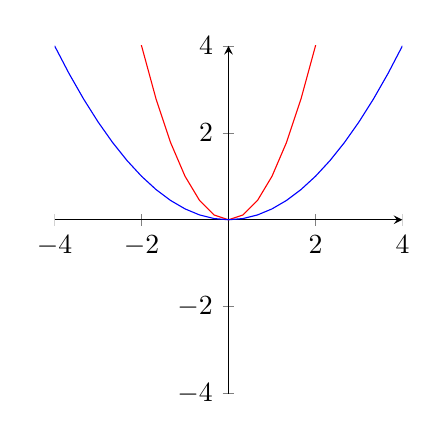
\begin{tikzpicture}
\begin{axis}[
    axis lines=middle, width=6cm, height=6cm, ymin=-4, ymax=4, ytick={-4, -2, 2, 4}, xmin=-4, xmax=4, ytick={-4, -2, 2, 4}
]
\addplot[domain=-4:4, color=red]{x^2};
\addplot[domain=-4:4, color=blue]{(0.5*x)^2};
\end{axis}
\end{tikzpicture}
\end{center}

\textbf{Vertical} dilations are represented by multiplying the output by a constant factor.

\begin{equation*}
    g(x) = a\cdot f(x)
\end{equation*}

\begin{center}
\begin{tikzpicture}
\begin{axis}[
    axis lines=middle, width=6cm, height=6cm, ymin=-4, ymax=4, ytick={-4, -2, 2, 4}, xmin=-4, xmax=4, ytick={-4, -2, 2, 4}
]
\addplot[domain=-4:4, color=red]{x^2};
\addplot[domain=-4:4, color=blue]{2*x^2};
\end{axis}
\end{tikzpicture}
\end{center}

A value of $a > 1$ results in compression whereas a value of $0 < a < 1$ results in an expansion. This is true for both horizontal and vertical dilations. Keep in mind that if $a < 0$, a reflection is at play too.

\section{Operations and Compositions}

\subsection{Operations}
Similarly to how operations like addition and multiplication can be applied to existing numbers to create new numbers, they can also be applied to functions to create new functions. Below are the effects of applying various operations to two functions:
\renewcommand{\arraystretch}{1.25}
\begin{table}[H]
    \centering
    \begin{tabular}{p{2cm} p{10cm}}
    Sum & $(f+g)(x) = f(x) + g(x)$ \\
    Difference & $(f-g)(x) = f(x) - g(x)$ \\
    Product & $(f \cdot g)(x) = f(x) \cdot g(x)$ \\
    Quotient & $(\frac{f}{g})(x) = \frac{f(x)}{g(x)}$, provided $g(x)\neq0$\\
    \end{tabular}
\end{table}
\renewcommand{\arraystretch}{1}
The domain of a function created by applying an operation on two component functions is the intersection of the domains of the component functions. In the case of a quotient operation, the domain on which the dividend function equals 0 must be ommitted. 

\subsection{Compositions}
The \textbf{composition} of two functions refers to using the output of one function as the input of another. It is written as follows: $(f \circ g)(x) = f(g(x))$. As can be seen, first the function $g(x)$ is applied to input $x$, and the resulting value is used as input for the function $f(x)$. The domain of $(f \circ g)(x)$ is the domain on which $g(x)$ is part of the domain of $f(x)$. In other words, the domain consists of all points in the domain of the first function that map to values that are also in the domain of the second function.

\section{Inverse Functions}

\subsection{Definition}
The \textbf{inverse} of a function $f(x)$, written as $f \textsuperscript{-1} (x)$ and equivalent to a reflection over the line $y=x$, refers to a function $g(x)$ that swaps every input and output value of $f(x)$. In other words, if $g(x)$ is the inverse of $f(x)$, then for every $a$ in the domain of $f(x)$, $f(a) = b$ and $g(b) = a$. 

\subsection{Finding the Inverse}
Given an equation describing $y$ in terms of $x$, the inverse can be found by algebraically rewriting the equation to describe $x$ in terms of $y$. 

Once again, there is some degree of nuance present in the relationship between equations and functions. The first equation may not be a function at all; it may fail the vertical line test. Likewise, the inverse equation may not be a function either. Any parabola is an example of this. Take the parent function $y=x^2$: the inverse equation(s) $x=\pm \sqrt{y}$ is not a function, as it can return two possible outputs for any given input.

\subsection{Existence}

An easy way to tell if a function has an \textbf{inverse function}, that is, an inverse relation that is also a function, is the horizontal line test:

A function $f(x)$ has an inverse function $g(x)=f \textsuperscript{-1} (x)$ \textbf{if and only if} every horizontal line intersects the graph of $f(x)$ at no more than one point. 





\end{document}

\end{document}
